\begin{figure*}[!t]
  \centering
  \captionsetup[subfloat]{font=scriptsize}
  \subfloat[Introduced attention disturbances (absolute difference) after filtering pre-softmax attention logits $\!<\!0$.]{
  \footnotesize
  \label{fig:teaser_attn_diff}
    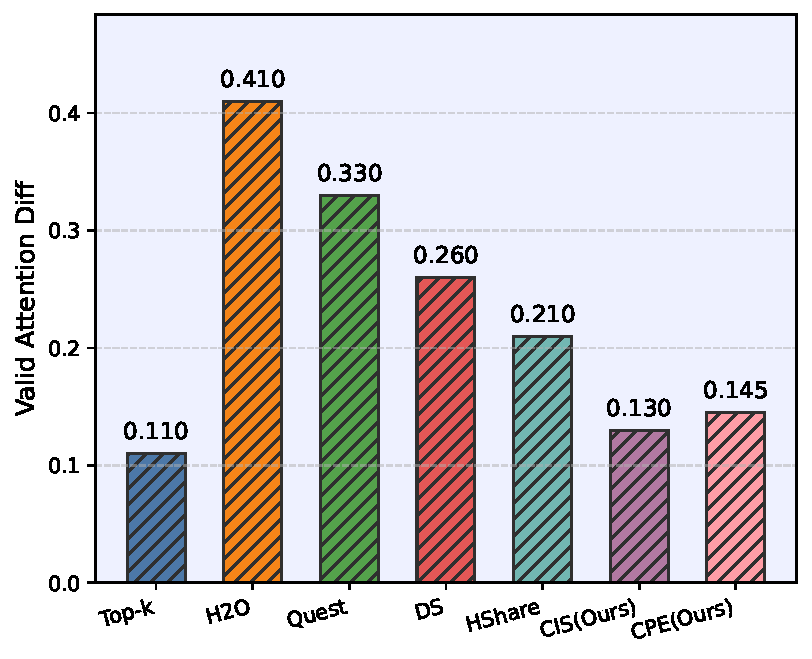
\includegraphics[width=0.305\textwidth]{assets/teaser/attn_diff.pdf}
  }\hfill
  \subfloat[Introduced absolute differences between original attention outputs.]{
  \footnotesize
  \label{fig:teaser_latent_diff}
    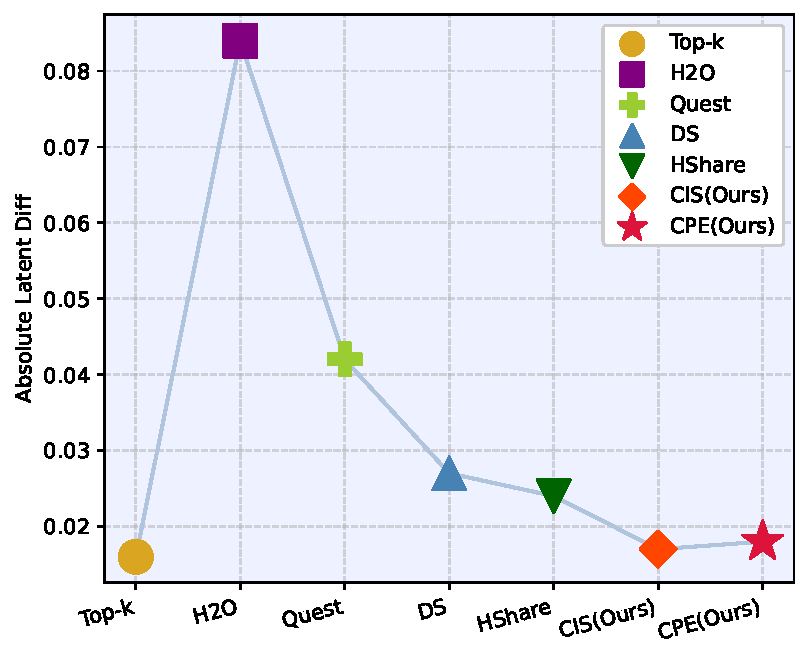
\includegraphics[width=0.305\textwidth]{assets/teaser/latent_diff.pdf}
  }\hfill
  \subfloat[Overall comparisons on accuracy-consumption trade-offs among state-of-the-art baselines.]{
  \footnotesize
  \label{fig:teaser_overall_comp}
    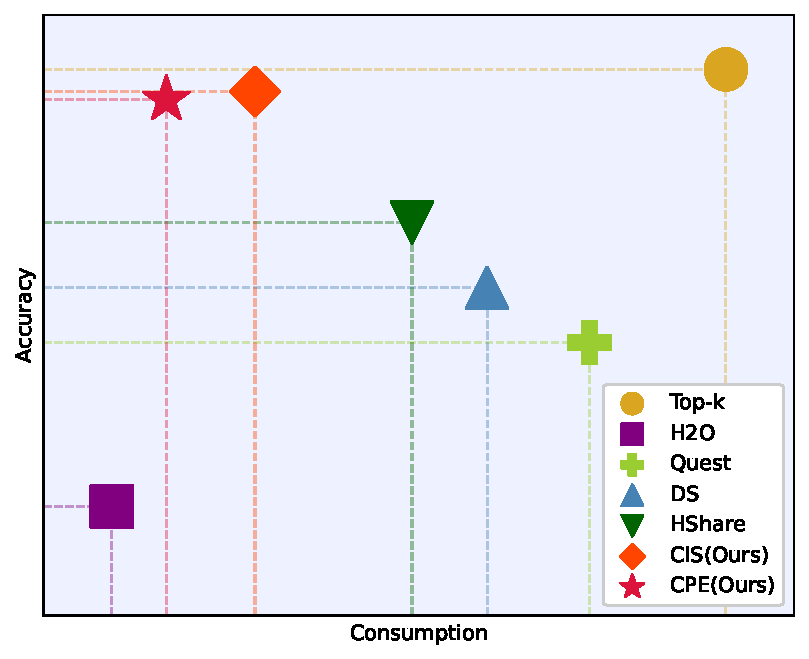
\includegraphics[width=0.305\textwidth]
    {assets/teaser/overall_comp.pdf}
  }
  \vspace{-0.05in}
  \caption{\textbf{Overall analysis of performance and efficiency}. Across induced attention-approximation error and accuracy-efficiency trade-offs, our method consistently surpasses prior SOTA approaches and closely tracks the top-$k$ oracle for optimal KV compression accuracy.}
  \label{fig:teaser}
  \vspace{-0.1in}
\end{figure*}





\iffalse
\begin{figure*}[!t]
    \centering
    \subfigure[Overall comparisons on accuracy and resource consumption among existing techniques.]{
        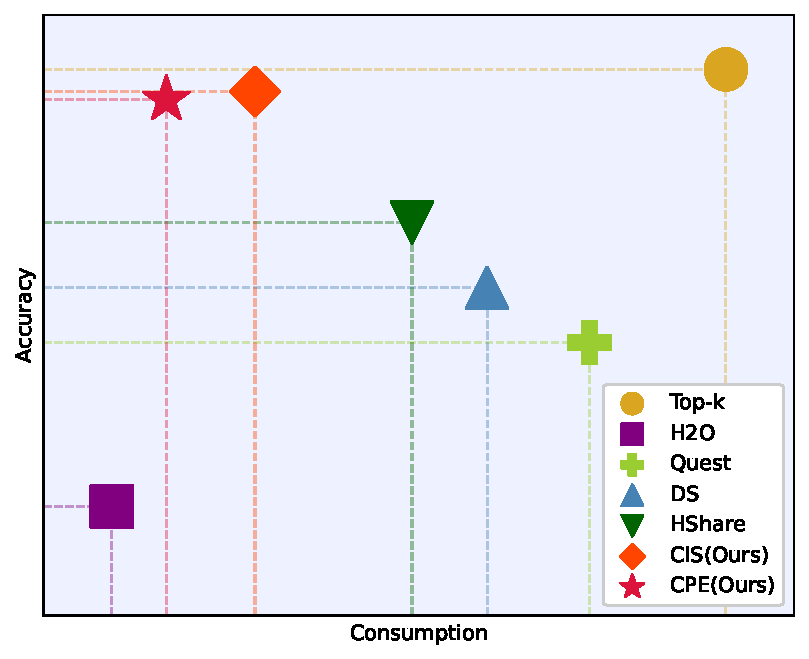
\includegraphics[width=0.305\textwidth]{assets/teaser/overall_comp.pdf}
        %\label{fig:teaser_overall_comp}
    }
    \hfill
    \subfigure[Introduced attention disturbances after filtering attention lgits $<0$.]{
        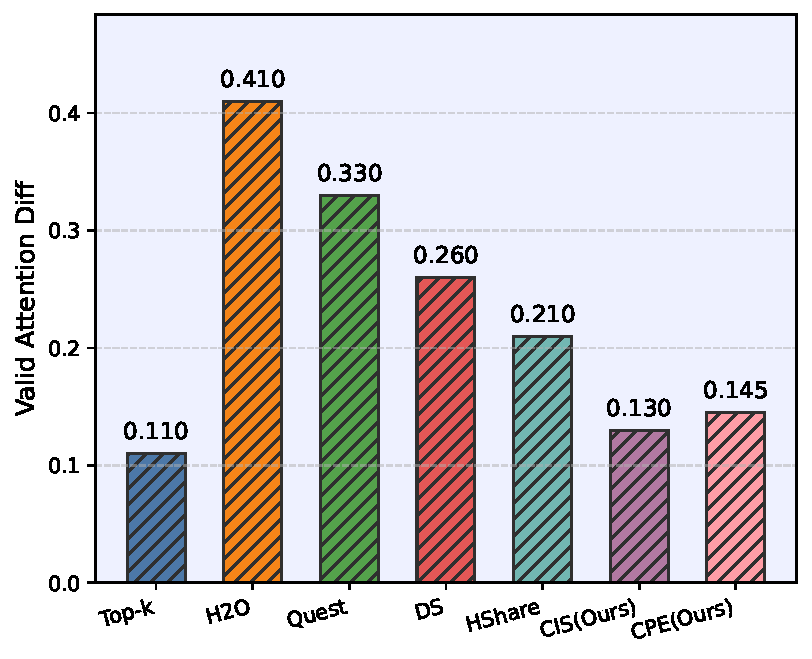
\includegraphics[width=0.305\textwidth]{assets/teaser/attn_diff.pdf}
        %\label{fig:teaser_ppl_elim}
    }
    \hfill
    \subfigure[Introduced absolute differences between original attention outputs.]{
        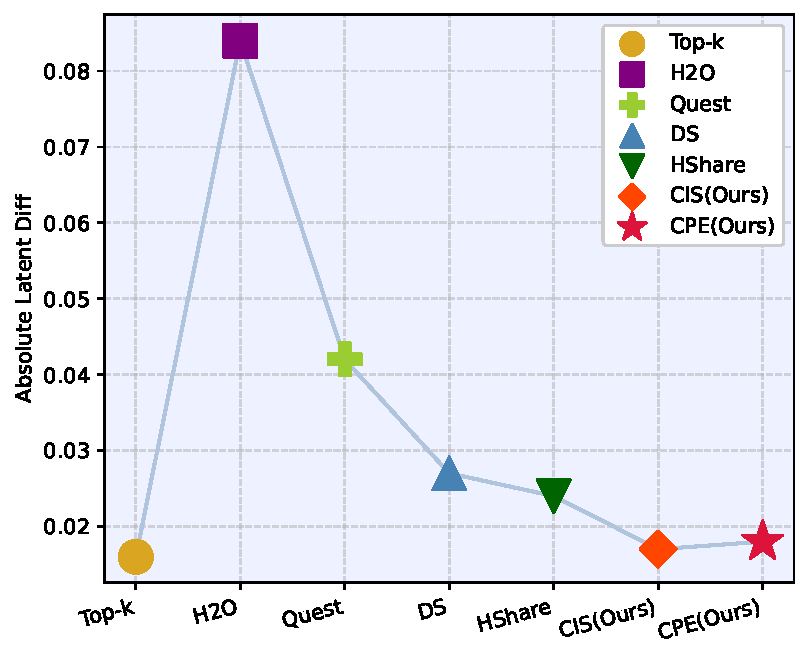
\includegraphics[width=0.305\textwidth]{assets/teaser/latent_diff.pdf}
        % \label{fig:teaser_acc_elim}
    }
    \vspace{-0.1in}
    \caption{Analysis of attention sparsity and its impact. (a) Attention is highly sparse across layers. (b) Perplexity maintains stable when large amounts of low-magnitude attention are eliminated. (c) Accuracy remains robust to large-scale attention pruning.}
    \label{fig:teaser}
    \vspace{-0.1in}
\end{figure*}
\fi




\iffalse
%------------------------------------------------------
\begin{figure*}[!t]
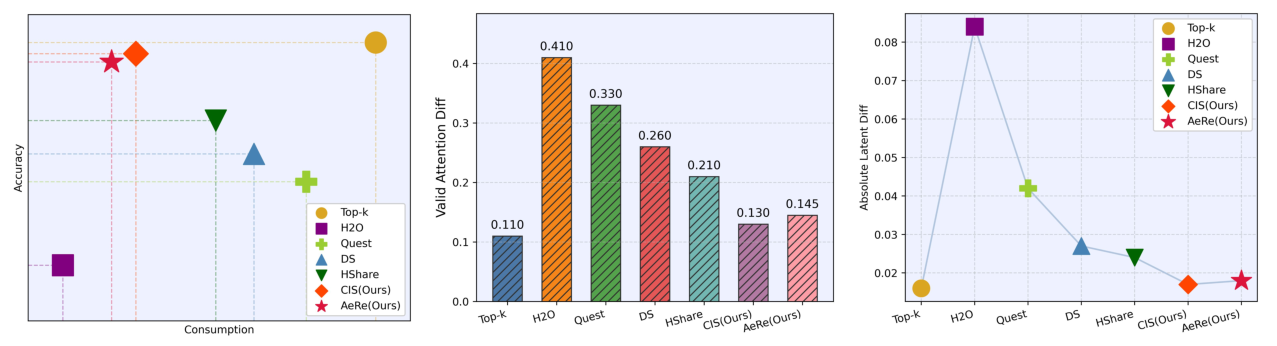
\includegraphics[width=1\textwidth]{assets/Teaser.pdf}
\centering
%\vspace{-1em}
    \caption{\textbf{Distribution of critical indices across heads and layers in LLaMA2-Chat-7B.} We highlight the critical indices in \textcolor{red}{red} and select the critical clusters (\textcolor{green!60!black}{green circles}, without local key tokens) within a range of consecutive queries (\textcolor{violet}{purple box}). Although not strictly contiguous, the critical key indices consistently form stable and dense clusters across multiple heads and layers.}
    \label{fig:teaser}
    %\vspace{-1.5em}
\end{figure*}
%------------------------------------------------------
\fi